\subsection{Electrical Power System}

The Electric Power System of the satellite must provide and manage the energy generated efficiently in order to have all the systems operating under normal conditions. The Electrical Power System of a Cubesat is, probably, the most fundamental requirement of the satellite payload, since its failure would result in the mission failure. The functions of the EPS are to control and distribute power to the Cubesat, to suppy a continuous source of electrical power for through the lifetime of the mission, to protect the satellite against bus failiures and to monitor and communicate the system status to the on-board computer. The role of the EPS is very diverse and the following subsystems have to be analyzed in detail.

\begin{figure}[h]
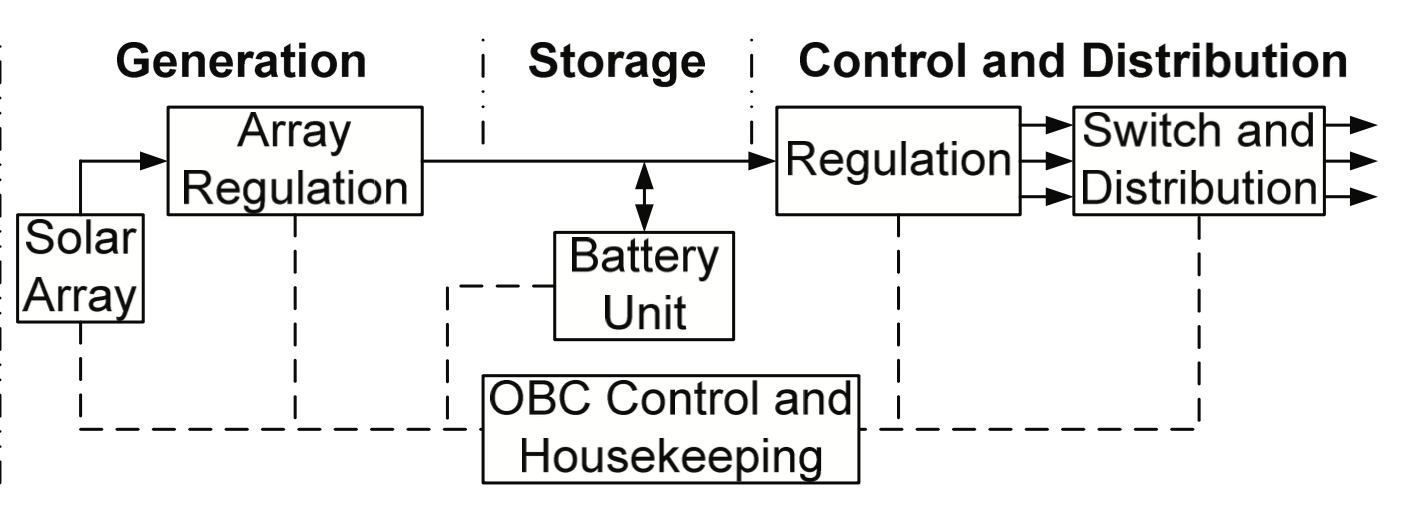
\includegraphics[scale=0.6]{./sections/SatelliteDesign/images/EPSschematics}
\centering
\caption{Basic schematics of the EPS \cite{epsbasics}}
\end{figure}

\subsubsection{Solar arrays}

\paragraph{}The primary source of electrical power has to be photovoltaic cells, given the size of the CubeSat. The photovoltaic cells will collect and convert the energy of the sun into electrical energy. Since they are main power source, they have to be correctly selected to prevent failure. Among the characteristics we seek for our mission, we are looking specially wheter the solar cell has a decent amount of power collection, low mass, protective radiation shield, deployment system, great temperature range and compatibility with the other systems.\\
The selected option for the Astrea mission will be a set deployable solar panels provided by EXA (Agencia Espacial Civil Ecuatoriana). These panels are low mass (135g each), have a protective radiation shield (NEMEA Anti Radiation Shield protects the solar panels of EM, High Gamma, X-Ray, Alfa, Beta and low neutron radiation), a very high temperature range (from -80 to 130ºC), a gentle release and deployment with artificial muscles (developed by EXA) and provide a power of 16.8W each (19.2V@0.5A). \\
Every cubesat will have 6 deployable solar panels providing it with 100.8W of power to supply peak demands while it is operating. Additionally, it is worth mentioning that these solar arrays are compatible with the hardwared used in each of the satellites.



\subsubsection{Batteries}

\paragraph{}	Batteries are vital for a proper mission operation. They will provide the spacecraft subsystems with the power needed when the solar arrays are working less efficiently or not properly. Astrea is looking for decent capacity batteries (because the subsystems will not usually require a peak power and the batteries are just an emergency system), operating at the desired voltages and currents and 

\subsubsection{Power management}

\subsubsection{Study of the commercial available options}
Several commercial options have to be studied. The table provided below organizes some information about the different options purchased.

\begin{longtable}{| l | r | r | }
\hline
\rowcolor[gray]{0.80}	\textbf{Brand and model} &  \textbf{Features and description}     & \textbf{Money (\euro)}   \\
\hline
\endfirsthead

	   ~Solar arrays & EXA (Agencia Espacial Civil Ecuatoriana & 17000) \\
	   ~Truñaas 1 & EMPTY & 20000 \\
	   ~Cuescas 1 & EMPTY & 20000 \\
	\hline

\caption{Options studied}
\label{epsoptionstable}
\end{longtable}

Of all the options in \ref{epsoptionstable}, we have chosen the following options.
